\documentclass[10pt]{beamer}

\usepackage{graphicx}
\usepackage{proof}
\usepackage{booktabs}
\usepackage[scale=2]{ccicons}

\usetheme[everytitleformat=regular, progressbar=foot]{m}
\usefonttheme[onlymath]{serif}

% Macros
\let\oldemptyset\emptyset
\let\emptyset\varnothing
\newcommand{\case}{\text{ case }}
\newcommand{\of}{\text{of }}
\newcommand{\yields}{\multimap}
\newcommand{\steps}{\Rightarrow}
\newcommand{\lquine}{\left\ulcorner}
\newcommand{\rquine}{\right\urcorner}
\newcommand{\capa}{\text{cap}}
\newcommand{\ptr}{\text{ptr }}


\title{Mechanical proof of type soundness for $L^3$}
\subtitle{$L^3$: \textit{The Linear Language with Locations}}
\author{Michael Sproul}
\date{}
\institute{
    Supervisor: Ben Lippmeier\\
    University of New South Wales
}

\begin{document}

\maketitle

\section{Introduction}

\begin{frame}{What?}

\begin{enumerate}
\item Model the \textit{type system} and \textit{semantics} of a small programming language as a formal mathematical system.
\item Prove that the programming language is ``well-behaved" -- \textit{sound}.
\end{enumerate}
\end{frame}

\begin{frame}
{Motivation}

Programming languages are complicated, lots of interacting features.

We want to:

\begin{itemize}
\item Eliminate or minimise undefined behaviour.

% Do closures work well with exceptions?
\item Ensure that language features interoperate without creating unsoundness.

\item Provide a solid foundation for software verification.

\end{itemize}
\end{frame}

\begin{frame}
{Motivation}

Formalised language semantics are a prerequisite for:

\begin{itemize}
\item Proofs about programs. \textit{seL4}, verified crypto.
    \begin{itemize}
    \item Security, correctness.
    \end{itemize}
\item Trust-worthy compilers. \textit{CompCert}.
\item Sanity whilst programming?
\end{itemize}
\end{frame}

\section{Background}

\begin{frame}{Contraction and Weakening}

In regular* logic there are two rules that allow assumptions to be discarded, or introduced from nowhere:

$$
\infer[\text{Contraction}]{\Gamma, A \vdash B}{
	\Gamma, A, A \vdash B
}
\qquad
\infer[\text{Weakening}]{\Gamma, A \vdash B}{
    \Gamma \vdash B
}
$$

*regular = classical/intuitionistic/constructive

\end{frame}

\begin{frame}{Contraction and Weakening}

Every logic corresponds to a type system, so we have...

\begin{eqnarray*}
\infer[\text{Contraction}]{\Gamma, x : A \vdash u[x/y, x/z] :: B}{
	\Gamma, y : A, z : A \vdash u :: B
}
\qquad
\infer[\text{Weakening}]{\Gamma, x : A \vdash y :: B}{
    \Gamma\vdash y :: B
}
\end{eqnarray*}

Without contraction, variables can only appear once in a term.
% Note: This is because concatenation of environments requires distinct variables.

Without weakening, all variables in the context must be used in the term.

[Wadler 1991, 1993]

\end{frame}

\begin{frame}{Linear and affine type systems}

\begin{itemize}
\item \textbf{Linear type system:} Contraction and weakening banned -- every value used \textit{exactly} once.
\item \textbf{Affine type system:} Contraction banned, weakening allowed -- every value used \textit{at most} once.
\end{itemize}

From linear logic [Girard 1986] and affine logic respectively.

\end{frame}

\begin{frame}{Retaining intuitionistic behaviour}

Linear type systems allow some terms to be treated in the normal intuitionistic way, via the bang operator, (!).

\begin{eqnarray*}
\emptyset \vdash \lambda \langle x' \rangle . \case x' \of !x \rightarrow \langle !x, !x \rangle :\text{ } !A \yields (!A \otimes !A)
\end{eqnarray*}

Derivable using a version of contraction that requires \textit{non-linear} assumptions [Wadler 1993].
% Note: The case statement is required to coerce an assumption of the form x': !A to [x: A].

\end{frame}

\begin{frame}

\frametitle{Why bother?}

Several languages use type systems based on linear logic to provide useful features:

Mutation without sacrificing referential transparency (Clean).
% Note: Unique references to memory permit destructive updates.

\begin{figure}[h]
\centering
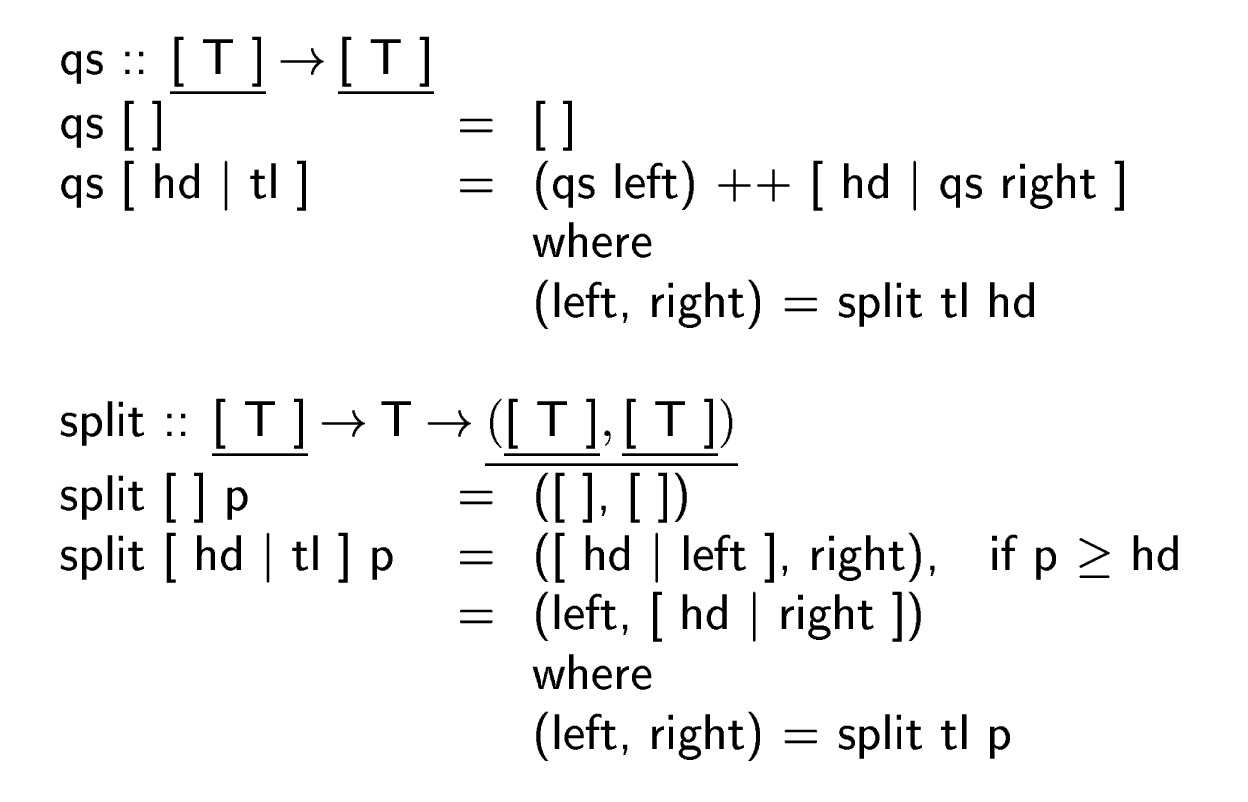
\includegraphics[width=250px]{Clean_Quicksort.png}
\label{}
\end{figure}
\end{frame}

\begin{frame}[fragile]{Why bother?}

Memory safety without garbage collection --\\
	Cyclone [Grossman et al. 2005], Rust.

\begin{verbatim}
fn main() {
    // Heap allocated vector - but we don't need to free it!
    let mut v = Vec::new();

    for i in 0 .. 200 {
        v.push(i * i);
    }

    println!("{:?}", v);
}
\end{verbatim}

\end{frame}

\begin{frame}[fragile]{Uniqueness typing}

Linear (and affine) typing aren't quite enough to guarantee unique references to values.

\textit{Dereliction} allows a non-linear value to be used as a linear one.

\begin{eqnarray*}
\lambda x \cdot x : & \alpha^\times \rightarrow \alpha^\odot & \text{(linear dereliction)}\\
\lambda x \cdot x : & \alpha^\odot \rightarrow \alpha^\times & \text{(uniqueness removal)}
\end{eqnarray*}

In a pure linear (or affine) type system, uniqueness of linear values therefore isn't guaranteed [de Vries 2008].
\end{frame}

\begin{frame}{Uniqueness typing}

\begin{itemize}
\item \textbf{Linear/affine typing}: Linear values \textit{will not} be duplicated at any point in the future.
\item \textbf{Uniqueness typing}: Linear values \textit{have not} been duplicated at any point in the past.
\end{itemize}

\end{frame}

\begin{frame}{Uniqueness typing via attributes}

Edsko de Vries designed a system that uses a uniqueness \textit{kind}, and a type constructor \texttt{Attr} which annotates a type as either unique or non-unique.

\begin{figure}[h]
\centering
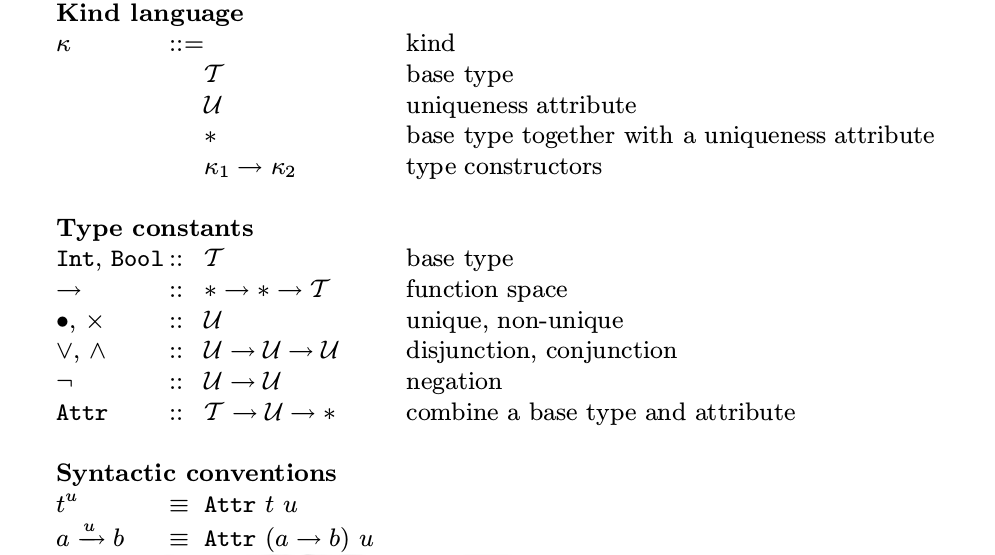
\includegraphics[width=300px]{de_Vries_attributes.png}
\label{}
\end{figure}
% Levity polymorphism?
\end{frame}

\begin{frame}{Uniqueness typing formalisation}
de Vries used Coq to prove soundness for his attribute-based type system.

\begin{itemize}
\item Locally nameless approach used for variable naming -- de Bruijn indices for bound variables and names for free variables.

\item \textit{The use of the locally nameless approach, and in particular the use of the Formal Metatheory library, meant that little of our subject reduction
proof needs to be concerned with alpha-equivalence or freshness.}

\end{itemize}
\end{frame}

\begin{frame}[fragile]{The \textbf{$L^3$} language}

Based on the linear lambda calculus, supporting \textit{strong updates} via a system of capabilities [Ahmed, Fluet, Morrisett 2001].

\begin{verbatim}
let val r = ref () in
   r := true;
   if (!r) then
     r := 42
   else
     r := 15;
   !r + 12
end
\end{verbatim}

\end{frame}

\begin{frame}{The \textbf{$L^3$} language}

Pointers can be shared, but require a \textit{capability} to be read, written or discarded. The capability is treated \textit{linearly}.

\begin{eqnarray*}
(\sigma, \text{new } v) \Rightarrow (\sigma \uplus \{l \mapsto v\},
	\lquine l, \langle \capa, \ptr l \rangle \rquine)
\\
(\sigma, \text{let } \lquine \rho, x \rquine = \lquine l, v \rquine \text{in } e)
	\Rightarrow
	(\sigma, e[l/\rho][v/x])
\end{eqnarray*}

Different from de Vries' system in that neither \textit{dereliction} nor removal of uniqueness is allowed.

\end{frame}

\begin{frame}{The \textbf{$L^3$} language}

Swapping a value can change its type:

\begin{eqnarray*}
(\sigma \uplus \{l \mapsto v_1\}, \text{swap cap } (\ptr l) \text{ } v_2)
	\Rightarrow
	(\sigma \uplus \{l \mapsto v_2\}, \langle \capa, v_1 \rangle)
\end{eqnarray*}

\begin{figure}[h]
\centering
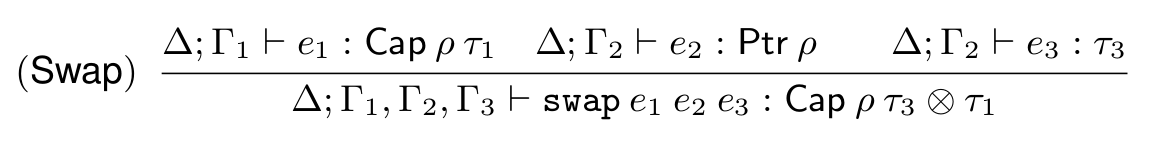
\includegraphics[width=300px]{L3_swap_rule.png}
\label{}
\end{figure}

\end{frame}

\begin{frame}{$L^3$ has a successor...}

[Ahmed, Fluet and Morrisett 2006] verified a system similar to $L^3$, with regions added on, \textbf{but without strong updates}.

\begin{itemize}
\item Twelf proof assistant, rather than Coq.
\item Higher-order abstract syntax -- host language binders used to describe object language binders.
\end{itemize}

Their conclusion from 2006 still seems to be true, \textbf{nobody has verified a system with strong updates yet}.

\end{frame}

\section{Proposal}

\begin{frame}{Proposal}

Model the operational semantics and type system of $L^3$ core using Coq, and prove \textit{progress} and \textit{preservation}.

$$
\infer[\text{Progress}]{\text{value } x \lor \exists x'.\text{ }x \steps x'}{
    \emptyset \vdash x : \tau
}
$$

$$
\infer[\text{Preservation}]{\emptyset \vdash x' : \tau}{
    \emptyset \vdash x : \tau \quad x \steps x'
}
$$

\end{frame}

\begin{frame}{What have I done so far?}

\begin{itemize}
\item Background reading on semantics and type theory.
\item Literature review - mostly papers on linear-logic based type systems.
\item Coq proofs of type soundness for simple variants of the lambda calculus, via \textit{Software Foundations} [Pierce 2015].
\end{itemize}
\end{frame}

\begin{frame}[fragile]{Software Foundations}

\begin{itemize}
\item STLC with let-bindings, fixed points, sum types and product types.
\item \textit{Globally shared names for variables} rather than HOAS, de Bruijn indices or locally nameless.

\begin{verbatim}
Lemma substitution_preserves_typing :
  forall Gamma x U t v T,
    extend Gamma x U |- t \in T ->
    empty |- v \in U   ->
    Gamma |- [x:=v]t \in T.
\end{verbatim}

\end{itemize}
\end{frame}

\begin{frame}{Approaches to naming}

SF avoids name capture by only permitting substitution of closed terms.

For $L^3$ I'll need to pick a better approach to variable naming.
% Need an approach that allows fresh names to be easily generated.

\begin{itemize}
\item Higher-order Abstract Syntax (HOAS).
\item de Bruijn indices [de Bruijn 1972].
\item Locally nameless, as used by [de Vries 2008].
\end{itemize}
\end{frame}

\begin{frame}{Schedule}

Before Week 12 (literature review deadline):

\begin{itemize}
\item Investigate approaches to variable binding (3 weeks).
\item Finish reading and summarising papers (also 3 weeks).
\end{itemize}

\pause

Over summer (3 months $\approx$ 12 weeks total):

\begin{itemize}
\item $L^3$'s operational semantics and type system in Coq (2 weeks).
\item Prove progress (4 weeks).
\item Prove preservation, and related lemmas (6 weeks).
\end{itemize}

Definitions may need tweaking along the way.
\end{frame}

\begin{frame}{Schedule}

Next semester (12 weeks):

\begin{itemize}
\item Finalise proofs completed over the summer break (6 weeks).
\item Write-up results and findings (6 weeks).
\end{itemize}

\end{frame}

\begin{frame}{References}
\begin{itemize}
\item \textit{Lambda Calculus Notation with Nameless Dummies} - N. G. de Bruijn (1972).
\item \textit{Linear Logic} - J. Girard (1986).
\item \textit{Higher-order abstract syntax} - F. Pfenning and C. Elliot (1988).
\item \textit{Linear types can change the world!} - P. Wadler (1991).
\item \textit{A taste of linear logic} - P. Wadler (1993).
\item \textit{Guaranteeing Safe Destructive Updates through a Type System with Uniqueness Information for Graphs} - S. Smetsers et al (1994).
\item \textit{$L^3$: A Linear Language with Locations} - A. Ahmed, M. Fluet, G. Morrisett (2001).
\item \textit{Linear Regions Are All You Need} - A. Ahmed, M. Fluet, G. Morrisett (2006).
\item \textit{Uniqueness Typing Simplified} - E. de Vries (2008).
\item \textit{Making Uniqueness Typing Less Unique} - E. de Vries (2008).
\item \textit{Software Foundations} - B. Pierce (2015).
\end{itemize}
\end{frame}

\begin{frame}
\begin{center}
\Large Thanks!
\end{center}
\end{frame}

\end{document}
